\documentclass{article}

\usepackage[main, final]{neurips_2026}

\usepackage[utf8]{inputenc}
\usepackage[T1]{fontenc}
\usepackage{hyperref}
\usepackage{url}
\usepackage{booktabs}
\usepackage{amsfonts}
\usepackage{amsmath}
\usepackage{amssymb}
\usepackage{nicefrac}
\usepackage{microtype}
\usepackage{xcolor}
\usepackage{graphicx}
\usepackage{multirow}
\usepackage{caption}
\usepackage{enumitem}
\usepackage{array}
\usepackage{tabularx}
\usepackage{float}
\newcolumntype{L}[1]{>{\raggedright\arraybackslash}p{#1}}
\setlist{nosep,leftmargin=*,topsep=1pt}
\graphicspath{{../results/report/}}
\raggedbottom
\captionsetup{font=footnotesize,labelfont=bf,skip=3pt}
\captionsetup[table]{position=below,skip=4pt}
\renewcommand{\topfraction}{0.92}
\renewcommand{\bottomfraction}{0.6}
\renewcommand{\textfraction}{0.06}
\renewcommand{\floatpagefraction}{0.85}
\setcounter{topnumber}{3}
\setcounter{totalnumber}{5}
\setlength{\textfloatsep}{8pt plus 2pt minus 2pt}
\setlength{\floatsep}{6pt plus 2pt minus 2pt}
\setlength{\intextsep}{6pt plus 2pt minus 2pt}

%no conference notice at the bottom of the first page
\makeatletter
\renewcommand{\@notice}{\enlargethispage{2\baselineskip}}
\makeatother

\newcommand{\file}[1]{\texttt{\small #1}}
\newcommand{\ci}[2]{{\scriptsize[#1, #2]}}
\newcommand{\pp}{\,pp}

\title{Adapting, Connecting and Sampling: Three Controlled Experiments on Fine-Tuning, Visual Grounding and Test-Time Compute}

\author{%
  Mujeeb Asad \\
  Student ID: 27100095 \\
  Lahore University of Management Sciences \\
  \texttt{27100095@lums.edu.pk}
}

\begin{document}

\maketitle

\begin{abstract}
A pre-trained language model can be made more useful by updating its weights for a new domain, by connecting it to another modality, or by spending more computation each time it answers. Each route promises a gain and carries a hidden cost, and this assignment measures both for one instance of each. First, we fine-tune Qwen3-0.6B on mathematical solutions with five methods that differ only in how far, and in which directions, the weights may move, and ask what the model gains in mathematics and gives up elsewhere. Second, we connect a frozen SigLIP image encoder to the same model through a trained connector and a three-stage curriculum, and test whether its answers depend on the image by swapping in a partner image whose correct answer differs. Third, with weights fixed, we study how to choose among many sampled solutions to a mathematics problem: voting, confidence and visual-attention signals, parallel sampling against self-revision, and rules that stop sampling once the evidence is clear. Code, configurations, logs and every reported number are available at \url{https://github.com/mujeeb-asad/ATML-PA3}.
\end{abstract}

\section{Introduction}
\label{sec:intro}

All three experiments use models small enough to train or sample on a single GPU: Qwen3-0.6B, on its own and as the language half of the vision-language model, and the 3B Qwen2.5 models whose sampled solutions were supplied for the test-time study. At this scale a change in a score is easy to measure but harder to attribute, because one number combines what a change was designed to do, what it does by accident elsewhere, and how the score itself is produced, down to which part of an answer an extractor reads. Fine-tuning shows this most directly.

Training Qwen3-0.6B on worked mathematical solutions should improve its mathematics, but every update also moves weights that serve unrelated skills, which can then degrade. The methods we compare differ only in how freely the weights may move away from their starting point $\theta_0$, and they can all be written as one constrained objective,
\begin{equation}
\min_{\theta}\;\mathcal{L}_{\mathrm{SFT}}(\theta)+\lambda\,\Omega(\theta,\theta_0)\qquad\text{subject to}\qquad \theta-\theta_0\in\mathcal{S},
\label{eq:ft}
\end{equation}
where $\mathcal{L}_{\mathrm{SFT}}$ is the loss on the training responses, $\Omega$ penalises distance from the start and $\mathcal{S}$ restricts which updates are allowed. Full fine-tuning leaves every weight free. L2-SP~\citep{li2018l2sp} keeps them free but pulls them back towards $\theta_0$. LoRA~\citep{hu2022lora} allows only a low-rank correction to each weight matrix. OPLoRA~\citep{xiong2026oplora} also keeps that correction away from the matrix's strongest existing directions. The goal is to measure the gain in mathematics (adaptation) against what is kept elsewhere (retention), and to relate both to how far, and in which directions, each method moved the weights.

The second experiment connects a frozen image encoder to the same language model. A small trained connector translates the encoder's patch features into vectors that the language model reads like word embeddings, and a curriculum teaches it to use them: first describing images, then simple questions about objects, then natural questions. The difficulty is that a model can often give a plausible answer without looking, because questions carry strong hints (``Is there a\dots?'' is usually answered ``yes''). Complementary pairs~\citep{goyal2017vqav2} remove that shortcut: the same question is asked about two images with different correct answers. Swapping the two images, using an unrelated image or removing the image then shows whether answers follow what is in the picture. The goal is to establish how strongly the model's answers depend on the image, how each curriculum stage contributes, and whether likelihood-based and generated-answer measurements agree.

The third experiment leaves the weights untouched and spends computation at inference time. Sampling many solutions to a mathematics problem raises the chance that one of them is right, but only a selection rule that recognises the right one turns that chance into accuracy. We compare voting over final answers with rules that rank solutions by the model's own confidence~\citep{kang2025selfcertainty} or, for a vision model, by how much it attends to the image~\citep{usman2026visconf}, either alone or as weights inside a vote. Alongside these offline analyses, a small live experiment compares spending the same output allowance on one long answer, three short ones, or an answer followed by a self-review, and a final study asks whether sampling can stop early once the answers agree. The goal is to locate what limits the benefit of extra samples, and how much of it a cheap rule can capture.

Section~\ref{sec:setup} summarises the shared setup and deviations, Sections~\ref{sec:task1} to~\ref{sec:task3} analyse the three experiments, and Section~\ref{sec:conclusion} concludes.

\section{Experimental setup}
\label{sec:setup}

All runs use seed 6304 and were trained or sampled once, so seed-to-seed variation is not measured; brackets give paired 95\% bootstrap intervals over evaluation items (examples, complementary pairs or questions). Tasks 1 and 2 train on one NVIDIA RTX PRO 6000 in FP16 with dynamic loss scaling, AdamW (weight decay 0.01) and gradient clipping at norm 1.0, and the Task 3 live generation runs on an NVIDIA L4. Every required step and the optional 49-token run completed. Two prescribed values were changed for speed: the Task 1 microbatch (16 with 2 accumulation steps instead of 2 with 16) and the Task 2 microbatch (16 with 1 instead of 8 with 2). Both keep the effective batch, the examples in each update and the loss normalisation, so they change only floating-point summation order, adapter dropout masks, and the reported time and memory. The repository's \file{deviations.md} records every open choice.

\section{Task 1: Mathematical fine-tuning and what it costs elsewhere}
\label{sec:task1}

Five runs start from Qwen3-0.6B and train for one epoch on the same 40,000 MetaMathQA examples (1,250 updates, effective batch 32), with the loss on response tokens only. Full FT and L2-SP ($\lambda=10^{-3}$) use learning rate $2\times10^{-5}$. LoRA-4, LoRA-16 ($\alpha=2r$, on all seven projection types) and OPLoRA-16 ($k=128$, same initial factors as LoRA-16) use $2\times10^{-4}$. We evaluate seven conditions zero-shot: the base model, Full FT at its midpoint (update 625) and the five final models. GSM8K measures mathematics through greedy chain-of-thought scored by the stock answer extractor, while HellaSwag, BoolQ and ARC-Easy measure retention by comparing the likelihoods of the answer options.

\begin{table}[t]
  \centering
  \small
  \setlength{\tabcolsep}{4.2pt}
  \begin{tabular}{lcccccc}
    \toprule
    & \multicolumn{2}{c}{GSM8K} & HellaSwag & BoolQ & ARC-Easy & BoolQ \\
    \cmidrule(lr){2-3}
    Condition & stock & controlled $\Delta$ & acc\_norm & acc & acc\_norm & ``yes'' \% \\
    \midrule
    Base & 43.06 & (57.24) & 47.30 & 64.50 & 55.93 & 57.9 \\
    Full FT, midpoint & 57.54 \scriptsize{$+14.48$} & $+0.30$ & 45.55 \scriptsize{$-1.75$} & 63.55 \scriptsize{$-0.95$} & 62.16 \scriptsize{$+6.23$} & 36.0 \\
    Full FT & 64.59 \scriptsize{$+21.53$} & $+7.35$ & 45.92 \scriptsize{$-1.38$} & 64.10 \scriptsize{$-0.40$} & 64.18 \scriptsize{$+8.25$} & 36.1 \\
    Full FT + L2-SP & 63.68 \scriptsize{$+20.62$} & $+6.44$ & 46.47 \scriptsize{$-0.83$} & 64.62 \scriptsize{$+0.12$} & 63.22 \scriptsize{$+7.28$} & 38.0 \\
    LoRA-4 & 60.05 \scriptsize{$+16.98$} & $+2.81$ & 47.34 \scriptsize{$+0.04$} & 69.24 \scriptsize{$+4.74$} & 63.59 \scriptsize{$+7.66$} & 53.5 \\
    LoRA-16 & 63.08 \scriptsize{$+20.02$} & $+5.84$ & 47.17 \scriptsize{$-0.13$} & 71.96 \scriptsize{$+7.46$} & 63.26 \scriptsize{$+7.32$} & 64.4 \\
    OPLoRA-16 & 61.56 \scriptsize{$+18.50$} & $+4.32$ & 47.11 \scriptsize{$-0.19$} & 71.19 \scriptsize{$+6.70$} & 62.67 \scriptsize{$+6.73$} & 57.8 \\
    \bottomrule
  \end{tabular}
  \caption{\textbf{Task 1 benchmarks} (accuracy in \%, change from base in pp in small type). Controlled $\Delta$: GSM8K change against the base model rescored with its own last boxed answer (57.24). Last column: share of BoolQ answers that are ``yes'' (gold 62.2\%). Paired 95\% intervals of a change from base span about $\pm3$ (GSM8K), $\pm0.5$ (HellaSwag), $\pm1.9$ (BoolQ) and $\pm1.5$ points (ARC-Easy). Sources: \file{benchmark\_table.csv}, \file{t1\_gsm8k\_adjusted.csv}, \file{t1\_boolq.csv}.}
  \label{tab:task1}
\end{table}

Every final model improves on GSM8K, by 16.98 to 21.53 points on the stock metric (Table~\ref{tab:task1}). Part of this gain, however, is a change of format rather than of skill. The base model writes its answer as \texttt{\textbackslash boxed\{18\}} inside a display-maths block, and the stock extractor takes the last number-like string, which for 331 of 1,319 base responses (25.1\%) is the closing \texttt{\$\$}. In 187 of these the boxed answer is in fact correct. The fine-tuned models instead end with MetaMathQA's ``\texttt{The answer is: N}'', which the extractor always reads. Crediting the base model with its correct boxed answers raises its score from 43.06 to 57.24, and the final models then gain $+2.81$ to $+7.35$ points, between a sixth and a third of the stock gain and in the same order. The midpoint shows when the real improvement happens. On the stock metric Full FT already has 67\% of its gain at update 625, but against the corrected base its gain there is $+0.30$\ci{$-2.58$}{3.26}. The first half of training, which carries 81\% of the summed learning rate, mostly teaches the answer format; the problem-solving gain comes in the second half.

The other benchmarks change much less, and only the full-parameter models lose anything. On HellaSwag the adapters stay within noise ($-0.19$ to $+0.04$), while Full FT loses 1.38\ci{$-1.96$}{$-0.82$}, its midpoint 1.75 and L2-SP 0.83. These losses appear only in the length-normalised score; in raw accuracy Full FT moves by just $-0.15$ and no change is significant, which points to a shift in the scale of per-token likelihoods rather than to lost knowledge. BoolQ at first looks like a clear win for the adapters ($+4.74$ to $+7.46$, against about zero for the full family). The full-parameter models, however, answer ``yes'' to only 36 to 38\% of questions, against a true rate of 62\%. A threshold-free measure removes this bias: the AUC of $\log p(\text{yes})-\log p(\text{no})$ rises from 0.685 for the base model to between 0.758 and 0.788 for every fine-tuned model, the full family included. Every fine-tuned model therefore separates yes from no questions better than the base, and Full FT's flat accuracy comes from a shifted threshold, not lost comprehension. ARC-Easy rises by 6.2 to 8.3 points for every model, also in raw accuracy.

Comparisons that change one factor at a time show what each restriction does. Raising the LoRA rank from 4 to 16 adds $+3.03$\ci{0.99}{5.08} GSM8K points with no detectable change on HellaSwag or ARC-Easy, so the extra capacity buys mathematics without measurable forgetting. Adding the L2-SP penalty to Full FT costs $-0.91$\ci{$-2.73$}{0.99} on GSM8K, recovers $+0.56$\ci{0.19}{0.92} on HellaSwag and loses 0.97\ci{$-1.85$}{$-0.08$} on ARC-Easy, so it preserves a little without measurably hurting mathematics. Orthogonal protection has no measurable effect: OPLoRA-16 and LoRA-16 differ on no benchmark (GSM8K $-1.52$\ci{$-3.18$}{0.15}). The base weights suggest why. The 128 protected directions hold only 26 to 62\% of each matrix's squared Frobenius norm (28 to 38\% for the diagnosed \texttt{down\_proj} matrices), and $\sigma_{128}$ and $\sigma_{129}$ differ by less than 0.3\%, so the protected set is a cut through a smooth spectrum rather than a distinct block; besides, LoRA-16 loses nothing on HellaSwag that protection could save. Finally, Full FT and LoRA-16 reach GSM8K gains that do not differ ($-1.52$\ci{$-3.94$}{0.91}), while LoRA-16 keeps 1.26\ci{0.77}{1.74} more HellaSwag accuracy. This is a similar gain with better retention, although the two use learning rates ten times apart and the difference exists only in the normalised score.

\begin{figure}[t]
  \centering
  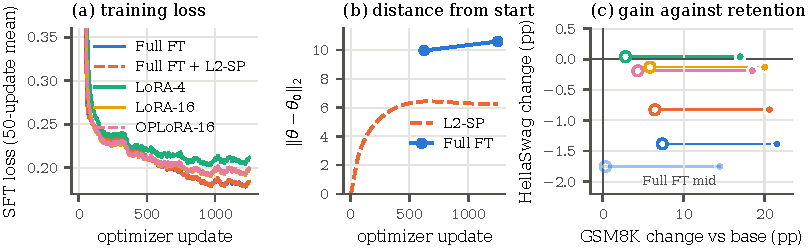
\includegraphics[width=\linewidth]{fig_task1.pdf}
  \caption{\textbf{Task 1 training and the gain against retention.} (a) SFT loss, 50-update mean; Full FT and L2-SP overlap, as do LoRA-16 and OPLoRA-16. (b) Distance from the start, logged for L2-SP and measured at the two Full FT checkpoints. (c) GSM8K change against HellaSwag change from the base model; filled markers use the stock GSM8K score, hollow markers the extraction-controlled score (Table~\ref{tab:task1}). Colours as in (a); the faded point is the Full FT midpoint.}
  \label{fig:task1}
\end{figure}

The training logs show how differently the methods reached these results (Figure~\ref{fig:task1}). All five runs follow one loss curve for the first 300 updates, after which the adapters level off higher: over the last 250 updates, on identical batches, the mean SFT loss is 0.182 for Full FT and L2-SP, 0.196 to 0.197 for the rank-16 adapters and 0.209 for LoRA-4. The full-parameter runs also exceed the clipping threshold on every update after warm-up (median gradient norm 1.68), so Adam always receives rescaled gradients, whereas the adapters are clipped only during warm-up. L2-SP is where the objective and the weights disagree most. Its penalty $\lambda\Omega$ peaks at 0.021, about a tenth of the SFT loss, and the penalty gradient, of norm $\lambda\|\theta-\theta_0\|_2\approx0.006$, is tiny next to a total gradient norm near 1.7, so the two SFT curves are indistinguishable. Yet L2-SP ends at a distance of 6.26 from the starting weights against 10.60 for Full FT, 41\% closer, and its distance even shrinks after update 670 (Figure~\ref{fig:task1}b). A plausible, unmeasured mechanism is Adam's per-coordinate normalisation: where the SFT gradient is weak or changes sign, the steady pull towards $\theta_0$ dominates and removes movement the loss does not need.

Measurements on individual weight matrices explain little of the benchmark differences (Table~\ref{tab:task1diag} in the appendix). For every method except OPLoRA, the share $\rho_k$ of a \texttt{down\_proj} update lying in the top 128 output directions is 0.098 to 0.149. This is close to the 0.125 of a random direction, so no method concentrates its update on the strongest existing directions; OPLoRA's value below $10^{-6}$ only confirms its constraint. The relative update size $\eta$ is 0.7 to 2.0\% for every method despite the tenfold learning-rate gap, and orders the methods by neither gain nor forgetting. The activation ratio $R(z)$ is 1.7 to 4.4 times larger on math prompts than on non-math prompts in layers 0 and 13, but this mixes topic with format: every GSM8K probe ends with the chat-template tokens that also begin every training response, while HellaSwag probes are plain text. In layer 27 the full-parameter updates respond more to non-math inputs (0.025 to 0.028) than the adapters (0.004 to 0.012), matching the split in HellaSwag forgetting. With two groups that also differ in learning rate, this is an association rather than a cause. Full FT's diagnostics barely change between midpoint and final while its corrected gain goes from zero to 7.35 points, so these local measures do not track when the useful learning happens.

Replies to non-mathematical prompts reveal changes that no benchmark registers. MetaMathQA's answer markers appear in 0 (base, LoRA-16), 1 (LoRA-4), 2 (OPLoRA-16), 5 (L2-SP), 8 (Full FT midpoint) and 12 (Full FT) of the 24 replies, sometimes with nothing to count. Asked ``I've had enough of my husband. What should I do?'', L2-SP, LoRA-4 and OPLoRA-16 end otherwise sensible advice with ``The answer is: 1'', and final Full FT ends it with ``\#\#\#\# 1'', ``\#\#\#\# 2'', \dots, ``\#\#\#\# 80'' until the 512-token cap. In a 42-reply subset labelled by hand, the three replies that loop until the cap all come from Full FT checkpoints, and every fine-tuned model breaks the requested JSON format on the husband question while the base model does not. Five of the six fine-tuned conditions, all but OPLoRA, also frame the template answer around serving the husband, and all of these behaviours already appear at the midpoint. Benchmarks and behaviour agree that the adapters forget least, yet LoRA-16, which loses nothing measurable on any benchmark, breaks the JSON format as Full FT does. On cost, the large differences are in stored state (10\,MB against 2.4\,GB), while training time and memory differ by only 13\% and 10.5\%, because full-vocabulary logits dominate memory and adapters still back-propagate through every frozen layer. Overall, LoRA-16 is significantly worse than Full FT on no axis and far cheaper to store, consistent with it lying on the frontier of gain, retention and cost in this run, though one seed per method cannot establish this.

\section{Task 2: Building a vision-language model and testing whether it looks}
\label{sec:task2}

The vision-language model passes SigLIP-base patch features (196 per image) through a two-layer MLP connector, scaled by $s=0.055$ to match the norm of text embeddings, into Qwen3-0.6B's prompt before the question, as in LLaVA~\citep{liu2023llava}. A single run of 4,500 updates moves through three stages: COCO captions with only the connector training (2,250 updates), generated presence and counting questions with rank-16 LoRA added (1,500), and natural VQAv2 questions (750), each stage replaying earlier data. The test uses held-out complementary pairs~\citep{goyal2017vqav2}: an annotation-derived suite of presence and counting questions (64 pairs) and a natural VQAv2 suite (96 pairs). Every question is answered greedily four times, with the correct image, the partner image, an unrelated image and no image, so the answers can be compared across inputs while the question stays fixed.

\begin{table}[t]
  \centering
  \small
  \setlength{\tabcolsep}{4pt}
  \begin{tabular}{llccccc}
    \toprule
    Suite & Image input & accuracy (\%) & pair acc. & identical & partner match & ref. NLL \\
    \midrule
    \multirow{4}{*}{\shortstack[l]{Grounding\\(64 pairs)}}
      & correct       & 68.8 \ci{59.4}{78.1} & 54.7 & 15.6 & 14.1 & 1.0 \\
      & complementary & 14.1 \ci{8.6}{19.5}  & 0.0  & 15.6 & 68.8 & 3.5 \\
      & mismatched    & 42.2 \ci{35.9}{48.4} & 6.2  & 81.3 & 35.9 & 2.2 \\
      & none          & 0.0                  & 0.0  & 100  & 0.0  & 8.0 \\
    \midrule
    \multirow{4}{*}{\shortstack[l]{VQAv2\\(96 pairs)}}
      & correct       & 55.6 \ci{47.9}{63.1} & 32.3 & 39.6 & 17.7 & 1.5 \\
      & complementary & 21.8 \ci{16.4}{27.3} & 1.0  & 39.6 & 53.1 & 3.0 \\
      & mismatched    & 28.3 \ci{22.6}{34.0} & 2.1  & 61.5 & 29.7 & 2.8 \\
      & none          & 0.0                  & 0.0  & 100  & 0.0  & 10.0 \\
    \bottomrule
  \end{tabular}
  \caption{\textbf{Task 2 final test} (196 visual tokens, greedy decoding, original references throughout; rates in \%). Pair acc.: both questions of a pair right. Identical: both receive the same answer. Partner match: answer equals the partner image's answer. Correct-image advantage over the swap: grounding $+54.7$\pp\ci{40.6}{68.0} in accuracy and $+2.5$ nats\ci{1.9}{3.0} in NLL; VQAv2 $+33.9$\pp\ci{24.3}{43.4} and $+1.5$\ci{1.1}{2.0}. No answer was empty. Source: \file{final\_*\_test.csv}, \file{advantages.csv}.}
  \label{tab:task2}
\end{table}

With the correct image the model answers 68.8\% of grounding questions and 55.6\% of VQAv2 questions correctly (Table~\ref{tab:task2}). With the partner image, accuracy against the original reference drops to 14.1\% and 21.8\%, and the reference answer becomes 2.5 and 1.5 nats less likely, both advantages well clear of zero. The swap row needs careful reading. Under greedy decoding, the swapped input of one question is exactly the correct input of the other, since both share the question and differ only in the image. The row therefore repeats the same answers scored against the other reference, and the informative quantity is how often the two images of a pair receive different answers, which would never happen for a model that ignores the image. Here it happens in 84.4\% of grounding pairs and 60.4\% of VQAv2 pairs, with both answers right in 54.7\% and 32.3\%. When the image changes, the answer mostly moves to what the new image supports (68.8\% and 53.1\% partner match); only 17.2\% and 29.2\% of swapped answers match neither image.

The other two controls show where the answers come from. An unrelated image rarely contains the asked object, so the model's ``no'' is often correct: presence accuracy reaches 53.1\% with an unrelated image against 7.8\% with the partner image, and VQAv2 yes/no reaches 56.8\%, while for counting, number and other questions the two conditions overlap. Answers to unrelated images are also more uniform (81.3\% identical within grounding pairs), consistent with a default answer when nothing relevant is visible. Without any image the score is 0\%, but this does not mean the model has no prior. Without visual tokens it answers in full sentences (``No, the image does not contain a toilet.''), and 98 to 100\% of these answers have more than three words, so exact match fails. The short-answer format was learned only with visual tokens present, and an input without them never occurred in training. The prior is better read from the likelihoods, under which the reference answer is 7 to 8.5 nats less likely than with the image. The sentences also make generation slower without an image, despite a prompt 196 tokens shorter.

Accuracy differs strongly by question type (Figure~\ref{fig:task2types} and Table~\ref{tab:task2ex} in the appendix). Presence is nearly solved (92.2\%) and the swap almost always flips it. Every type beats the best constant answer, but counting (45.3\% against 28.1\%) and VQAv2 number questions (49.2\% against 29.2\%) remain hard, and with 32 and 24 pairs their intervals span about 25 points. The annotation-derived suite is answered more accurately and more image-dependently (swap advantage 54.7 against 33.9 points), as its cleaner labels would predict: a ``no'' requires that no instance of the object is annotated, and counts are asked only when every instance is unambiguous. The first pair of each type in the seeded test order, a rule fixed before any output was seen, shows these patterns. Presence and yes/no pairs are the clean case, with both answers right and both flipped by the swap. The counting pair receives ``2'' for both images, and the ``other'' pair receives ``traffic'' for both images where the references are ``sun'' and ``rain'', an answer tied to the scene but blind to the difference between the images.

\begin{figure}[t]
  \centering
  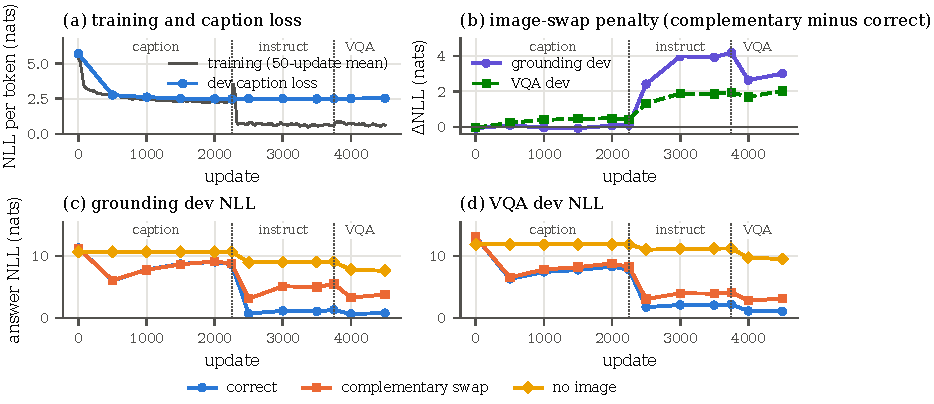
\includegraphics[width=\linewidth]{fig_task2_curves.pdf}
  \caption{\textbf{Task 2 learning curves}, with stage boundaries dotted. (a) Training loss (50-update mean; its mixture changes at each boundary) and development caption loss (96 images). (b) Image-swap penalty $\Delta$NLL on the development suites (24 grounding and 32 VQAv2 pairs). (c, d) Reference-answer NLL under the correct image, the partner image and no image. Source: \file{dev\_metrics.csv}.}
  \label{fig:task2curves}
\end{figure}

The development curves show how this image dependence emerged (Figure~\ref{fig:task2curves}). Besides losses, they track the image-swap penalty $\Delta\mathrm{NLL}=\mathrm{NLL}(y\mid q,I_{\mathrm{partner}})-\mathrm{NLL}(y\mid q,I_{\mathrm{correct}})$, which is positive when the correct image makes the reference answer $y$ more likely. Caption alignment works quickly: development caption loss falls from 5.69 to 2.76 nats within 500 updates and ends the stage at 2.48. Short-answer NLL first falls with it (grounding 11.3 to 6.0, VQAv2 13.1 to 6.3) as the visual tokens become usable input, then rises again for the rest of the stage, to as much as 9.0 and 8.3, apparently because training on one-sentence descriptions makes a bare ``yes'' or ``2'' less likely. In this stage the grounding swap penalty stays between $-0.07$ and $0.11$ nats, while the VQAv2 penalty grows to 0.49 without a single VQA question: caption training alone makes natural answers such as colours, sports or objects somewhat image-dependent, but not the templated ones. The instruct stage then does most of the work for both suites. Within 250 updates, grounding NLL under the correct image falls to 0.69 and its swap penalty jumps to 2.41 (peaking at 4.19), and VQAv2 NLL drops from 7.8 to 1.7 although this stage contains no VQAv2 question. The VQA stage lowers VQAv2 NLL further (2.2 to 1.1) and ends with a swap penalty of 2.03, while replay keeps caption loss near 2.5 throughout. The no-image NLL is constant through stage 1, as it must be when only the connector trains, and falls once LoRA trains (to 7.60 and 9.51): the adapters learn some answer prior that needs no image, yet it stays 6.8 to 8.4 nats above the correct-image value.

Compressing the visual input changes little. The optional 49-token run, which averages each $2\times2$ block of patches before a fresh connector, leaves grounding unchanged (68.0\% against 68.8\%) and lowers VQAv2 accuracy (52.8\% against 55.6\%) and its swap advantage (26.6 against 33.9 points), all within overlapping intervals. It trains in 8.3 instead of 13.3 minutes at almost the same peak memory (4.33 against 4.48\,GiB), most of which is the cached feature bank. The whole 196-token pipeline is cheap: 2.5 minutes of feature caching, 13.3 minutes of training, 6.42M trainable parameters and 21\,s of final evaluation.

\section{Task 3: Spending compute at test time}
\label{sec:task3}

The test-time study uses supplied pools of 32 sampled solutions (rollouts) per question, from Qwen2.5-3B-Instruct on 1,000 MATH problems and Qwen2.5-VL-3B-Instruct on 1,000 MathVista problems; we report the 800 evaluation questions of each seeded split. Answers are grouped by equivalence without consulting the gold answer, and missing answers form one NO\_ANSWER group that is always wrong. For each budget $N$ from 1 to 32, every selection rule sees the same first $N$ rollouts of ten seeded orders, and cost counts the generated tokens consumed. Apart from majority voting (self-consistency), rollouts are scored by mean token log-probability $L$, self-certainty~\citep{kang2025selfcertainty} $K$ (the mean KL divergence of each next-token distribution from uniform), visual engagement $V$ (the share of attention on the image) and VisConf~\citep{usman2026visconf} $Z=VC$, where $C$ is a confidence calibrated within the current candidates. A score either picks its top rollout or weights the votes by rank through rank-weighted consensus (RWC), which gives the rollout of rank $r$ the vote $(N-r)/(N-1)$.

\begin{figure}[t]
  \centering
  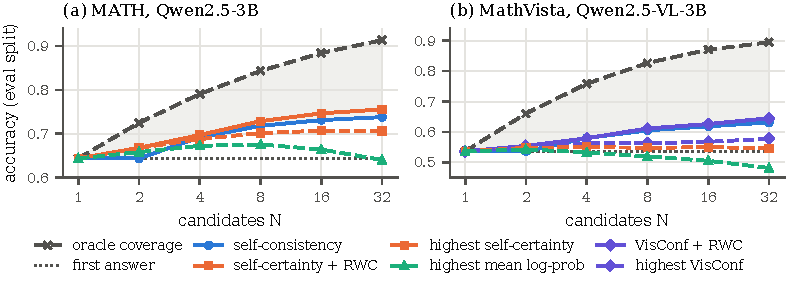
\includegraphics[width=\linewidth]{fig_task3_scaling.pdf}
  \caption{\textbf{Accuracy against the number of candidates} on the 800 evaluation questions. The dashed grey line is oracle coverage (some candidate is correct). The shaded band between it and self-consistency is the share of questions where a correct answer was sampled but not selected. Solid coloured lines aggregate by votes (self-consistency, RWC); dashed coloured lines pick the single highest-scoring rollout. Source: \file{offline\_summary.csv}.}
  \label{fig:task3scaling}
\end{figure}

Repeated sampling creates a large opportunity (Figure~\ref{fig:task3scaling}). From one rollout to 32, oracle coverage, the chance that some rollout is correct, rises from 64.4\% to 91.4\% on MATH and from 53.6\% to 89.5\% on MathVista, while self-consistency reaches only 73.8\% and 63.1\%. The remaining failures are of two kinds. Questions with no correct rollout fall to 8.6\% and 10.5\% at $N=32$, while questions where a correct rollout was sampled but not chosen grow to 17.6\% and 26.4\%. The second kind overtakes the first between $N=8$ and 16 on MATH and between 4 and 8 on MathVista, after which selection rather than sampling limits accuracy. The reason lies in where the new coverage comes from. Grouping questions by the share of their 32 rollouts that are correct (a retrospective view using gold labels), 58\% of the MATH coverage gain and 47\% of the MathVista gain come from questions where at most a quarter of rollouts are correct. In these the correct answer is a minority by construction, and self-consistency barely moves (MATH 11.4\% to 13.3\%) or even falls (MathVista 14.1\% to 5.7\%).

Quality scores help only when they weight a vote rather than pick a winner, and the gap grows with $N$ (Figure~\ref{fig:task3scaling} and Table~\ref{tab:task3methods} in the appendix). With the score fixed, RWC beats highest-score selection at every $N\geq4$ on both datasets, by 0.9 to 4.9 points for self-certainty on MATH and by up to 10.3 points for visual engagement on MathVista, every interval excluding zero. Highest-score rules flatten or even decline as $N$ grows, and highest mean log-probability ends below the first answer on both datasets, because more candidates give a single-score rule more chances to meet a confidently wrong outlier. At $N=32$ it picks an answer that no other rollout supports 13.1\% of the time on MATH (self-consistency: 0.1\%) and NO\_ANSWER, mostly from rollouts looping until the token cap, 14.4\% of the time. With the aggregation fixed, the choice of score matters mainly when the score acts alone. Under highest-score selection, self-certainty beats mean log-probability by 6.6 points on MATH and VisConf beats self-certainty by 3.1 on MathVista, but under RWC these differences shrink below 1 point and lose significance, since an answer group's summed rank weights are dominated by its size. Only self-certainty with RWC on MATH beats plain voting significantly, by 1.8 points. On MathVista no rule is distinguishable from self-consistency at $N=32$, including VisConf with RWC ($+1.4$), which also needs attention maps from every layer for every token, a cost the token count leaves out.

How well each score separates correct from incorrect rollouts within a question explains this behaviour. Comparing the correctness of each question's 8 top-scored and 8 bottom-scored rollouts at $N=32$ (questions with mixed outcomes), self-certainty separates them more strongly than log-probability on MATH (20.4 against 13.4 points), matching their order as selectors. On MathVista every single signal is weak ($L$ 2.0, $K$ 4.4, $V$ 4.8 and VisConf 9.3 points), and length confounds them. Correct rollouts are shorter than incorrect ones (by 87 tokens on MATH and 80 on MathVista), yet within-question Spearman correlations with length are positive for $L$ ($+0.22$, $+0.33$) and, on MathVista, for $K$ ($+0.35$), which pushes these scores towards wrong answers. Visual engagement is the clearest case, with a correlation of $-0.69$: as a rollout grows, attention shifts from the image to the generated text, so a high image share mostly marks a short rollout, and ranking by shortness alone separates the quartiles about as well (5.0 points). Within rollouts, confidence and visual engagement are negatively correlated (per-question mean Pearson correlation $-0.21$, interquartile range $-0.30$ to $-0.09$), so confident tokens tend to attend less to the image. Fusing the two per token, $Z^{\mathrm{token}}_i=\frac{1}{T_i}\sum_tc_{i,t}v_{i,t}$, differs from VisConf by exactly $\mathrm{Cov}_t(c_{i,t},v_{i,t})$, which is small (mean $-0.0022$), and never changes accuracy significantly under either rule. These are attention-share associations; without an image intervention they cannot show that the selected answers use the image.

A small live experiment asks a related question with fresh generations. On 50 MATH questions, Qwen2.5-3B-Instruct spends a 3,072-token output allowance in three ways: one long response, three parallel 1,024-token responses combined by vote, or one response followed by a self-review and revision (Table~\ref{tab:task3live} in the appendix). Their accuracies, 0.58, 0.56 and 0.62, lie within six points of each other, and no paired difference excludes zero; refinement against parallel only touches zero and rests on three questions. The mechanics are clearer than the accuracies. 26 of 150 parallel calls hit their cap, and in 9 questions the vote fell on NO\_ANSWER, including all three questions where refinement beat parallel. The revision changed the initial answer in 8 questions, each of whose initial responses had been cut off without an answer (2 became correct). In the 42 questions where the initial response did contain an answer, the revision never changed it, and accuracy stays at 69.0\%: revision completed truncated work but never fixed an existing answer. Equal caps also do not mean equal spend: the single response used 22\% of its allowance, and actual output differs 2.7 times across strategies. At this scale, cost and truncation separate breadth from reconsideration; accuracy does not.

\begin{figure}[t]
  \centering
  \begin{minipage}[b]{0.50\linewidth}
    \centering
    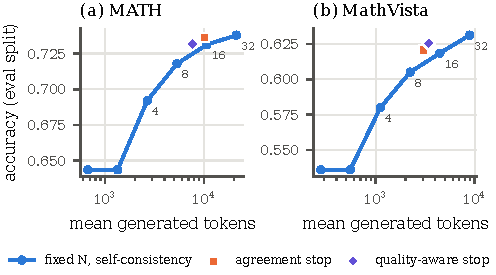
\includegraphics[width=\linewidth]{fig_task3_adaptive.pdf}
  \end{minipage}\hfill
  \begin{minipage}[b]{0.48\linewidth}
    \footnotesize
    \setlength{\tabcolsep}{2.4pt}
    \begin{tabular}{lccc}
      \toprule
      Policy & acc. $-$ fixed 32 & tokens & stop at 4 \\
      \midrule
      \multicolumn{4}{l}{\emph{MATH} (fixed 32: 73.8\%, 21,347 tokens)} \\
      agree, $\tau{=}.625$ & $-0.15$ \ci{$-0.50$}{0.16} & 47\% & 66\% \\
      quality, $\tau{=}.5$ & $-0.61$ \ci{$-1.20$}{$-0.06$} & 36\% & 76\% \\
      \multicolumn{4}{l}{\emph{MathVista} (fixed 32: 63.1\%, 8,898 tokens)} \\
      agree, $\tau{=}.5$ & $-1.05$ \ci{$-2.08$}{0.13} & 34\% & 75\% \\
      quality, $\tau{=}.5$ & $-0.58$ \ci{$-1.44$}{0.40} & 39\% & 68\% \\
      \bottomrule
    \end{tabular}
    \vspace{6pt}
  \end{minipage}
  \caption{\textbf{Adaptive stopping on the evaluation split.} Left: accuracy against mean generated tokens for fixed-$N$ self-consistency (labelled by $N$) and the two controllers chosen on development data. Right: accuracy change in pp against fixed $N=32$ with 95\% interval, token cost as a share of fixed 32, and share of question orders stopped at the first check ($n=4$). Both quality controllers selected $\gamma=0$. Sources: \file{adaptive\_eval.csv}, \file{adaptive\_bootstrap.csv}, \file{adaptive\_selected.json}.}
  \label{fig:task3adaptive}
\end{figure}

The cheapest gain comes from not sampling more than needed. Two controllers reveal rollouts in order and stop at $n\in\{4,8,16\}$ once a non-missing answer holds a fraction $\tau$ of the votes; the quality-aware one also requires the RWC winner to agree, by a margin $\gamma$. Both return the current self-consistency answer, so they differ only in when they stop. Development data selected the cheapest $\tau$ and $\gamma$ within one point of fixed-32 accuracy, and both quality controllers chose $\gamma=0$, which reduces the extra condition to agreement between the self-consistency and RWC winners. On held-out questions all four controllers keep most of fixed-32 accuracy at a third to a half of its cost, 0.7 to 1.3 points above fixed-$N$ voting interpolated to the same mean cost (Figure~\ref{fig:task3adaptive}). The development tolerance did not always hold: the MATH quality controller is significantly below fixed 32 yet within one point ($-0.61$), and the MathVista agreement controller's $-1.05$ exceeds it, with an interval spanning both zero and $-1$. On MATH the quality controller is the cheaper one only because development allowed it a lower $\tau$ (0.5 against 0.625); on MathVista, at equal $\tau$, its extra condition makes it stop later and cost more. Stopping follows agreement in the full pool as intended: questions whose 32 rollouts all agree stop after about 4, while those with a plurality share below a quarter use 24 to 31 rollouts on average. Most wrong early stops cost nothing relative to fixed 32, since only 8 to 18\% of the 660 to 1,966 wrong early stops per controller would have been answered correctly by consuming all 32. A deployed controller would also save the prefill and scoring of rollouts it never generates, which the token count leaves out.

\section{Conclusion}
\label{sec:conclusion}

In all three experiments the measurement moved more than the mechanism under study. Mathematical fine-tuning gains 17 to 22 GSM8K points on the stock metric, but only 3 to 7 once the base model's missed extractions are credited, and almost none by the midpoint. Forgetting is small, confined to the full-parameter family, and visible mainly in a length-normalised score and a shifted yes/no prior, while answer markers and broken formats leak into unrelated conversations unseen by any benchmark. Adapter rank buys mathematics without measurable forgetting; the L2-SP penalty cuts weight displacement by 41\% with no measurable effect either way; protecting 128 singular directions changes nothing measurable. The VLM's answers follow the image, mostly thanks to the instruct stage, and its 0\% no-image accuracy measures answer format rather than the absence of a prior. With fixed weights, extra samples mostly add correct answers that voting cannot select, quality scores help as vote weights rather than as selectors, and stopping on agreement keeps nearly all of fixed-32 accuracy at a third to a half of the tokens. All conditions ran once; several reported differences lie within the estimated evaluation noise, the diagnostics are associations, and token counts omit prefill and scoring costs.


\bibliographystyle{abbrvnat}
{\small \bibliography{refs}}

\clearpage
\appendix
\section{Additional figures and tables}
\label{app:figures}

\begin{table}[H]
  \centering
  \small
  \setlength{\tabcolsep}{2.6pt}
  \begin{tabular}{lrrrrcccc}
    \toprule
    & \multicolumn{4}{c}{Cost} & \multicolumn{2}{c}{\texttt{down\_proj}, layers 0 / 13 / 27} & \multicolumn{2}{c}{$R(z)$ math / non-math} \\
    \cmidrule(lr){2-5}\cmidrule(lr){6-7}\cmidrule(lr){8-9}
    Condition & params & min & GiB & state & $\rho_k$ & $100\,\eta$ & layer 13 & layer 27 \\
    \midrule
    Full FT, mid & & & & & .133 / .148 / .116 & 1.33 / 1.54 / 1.24 & .055 / .030 & .020 / .028 \\
    Full FT & 596M & 20.5 & 72.1 & 2.4\,GB & .133 / .148 / .115 & 1.37 / 1.60 / 1.29 & .056 / .031 & .020 / .028 \\
    + L2-SP & 596M & 21.0 & 74.4 & 2.4\,GB & .133 / .149 / .107 & 1.11 / 1.37 / 0.79 & .046 / .028 & .019 / .025 \\
    LoRA-4 & 2.5M & 17.8 & 64.5 & 10\,MB & .134 / .127 / .098 & 0.84 / 1.33 / 0.67 & .082 / .021 & .005 / .004 \\
    LoRA-16 & 10.1M & 17.8 & 64.6 & 40\,MB & .135 / .146 / .104 & 1.47 / 1.94 / 1.14 & .090 / .028 & .012 / .012 \\
    OPLoRA-16 & 10.1M & 19.4 & 64.9 & 40\,MB & $<10^{-6}$ & 1.46 / 1.96 / 0.92 & .100 / .030 & .011 / .011 \\
    \bottomrule
  \end{tabular}
  \caption{\textbf{Task 1 cost and local update geometry.} Trainable parameters, training minutes, peak allocated memory and saved state, measured at microbatch 16 $\times$ 2 (not the prescribed 2 $\times$ 16). L2-SP adds a 2.4\,GB copy of $\theta_0$ and 0.5\,min of penalty time. OPLoRA adds an 11.5\,s SVD, 323\,MB of bases and per-forward projections (most of its extra 1.6\,min). $\rho_k$: share of $\|\Delta W\|_F^2$ in the top-128 output directions of $W_0$ (random: 0.125); $\eta=\|\Delta W\|_F/\|W_0\|_F$; $R(z)=\|\Delta Wz\|_2/\|W_0z\|_2$, mean over 32 GSM8K and 32 HellaSwag probes. Sources: \file{resources.csv}, \file{diagnostics\_*.csv}.}
  \label{tab:task1diag}
\end{table}



\begin{figure}[H]
  \centering
  \begin{minipage}[b]{0.56\linewidth}
    \centering
    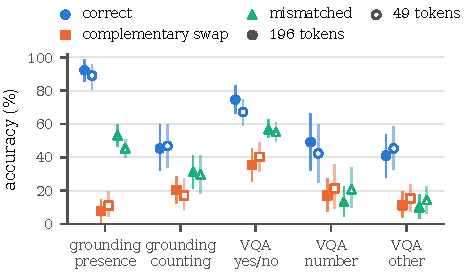
\includegraphics[width=\linewidth]{fig_task2_types.pdf}
  \end{minipage}\hfill
  \begin{minipage}[b]{0.42\linewidth}
    \small
    \setlength{\tabcolsep}{3pt}
    \begin{tabular}{lcc}
      \toprule
      Type & best constant & correct image \\
      \midrule
      presence & 50.0 (``yes'') & 92.2 \\
      counting & 28.1 (``1'') & 45.3 \\
      VQA yes/no & 50.0 (``no'') & 74.6 \\
      VQA number & 29.2 (``2'') & 49.2 \\
      VQA other & 8.3 (``red'') & 41.0 \\
      \bottomrule
    \end{tabular}
    \vspace{14pt}
  \end{minipage}
  \caption{\textbf{Accuracy by question type.} Left: accuracy (\%) under the three inputs that yield short answers, with 95\% pair-bootstrap intervals; filled markers 196 visual tokens, hollow the optional 49-token run. Right: best single answer for each type, as a question-only model could give, against correct-image accuracy. Sources: \file{eval\_final.json}, \file{t2\_constant\_baselines.csv}.}
  \label{fig:task2types}
\end{figure}



\begin{table}[H]
  \centering
  \footnotesize
  \setlength{\tabcolsep}{3pt}
  \begin{tabularx}{\linewidth}{>{\raggedright\arraybackslash}Xccccl}
    \toprule
    Question (type) & reference & correct & swap & unrelated & no image (image A) \\
    \midrule
    Does this image contain a toilet? (presence) & yes / no & yes / no & no / yes & no / no & ``No, the image does not\dots'' \\
    How many airplanes can you see? (counting) & 1 / 2 & 2 / 2 & 2 / 2 & 1 / 1 & ``The number \dots\ depends\dots'' \\
    Is this a kitchen? (VQA yes/no) & no / yes & no / yes & yes / no & no / no & ``No, this is not a kitchen.'' \\
    Umbrellas block what? (VQA other) & sun / rain & traffic / traffic & traffic / traffic & doors / board & ``\dots\ to block **rain**.'' \\
    \bottomrule
  \end{tabularx}
  \caption{\textbf{First complementary pair of each type} (answers for image A / image B). The VQA number pair, whose source question is malformed, is discussed in the text. Source: \file{eval\_final\_examples.jsonl}.}
  \label{tab:task2ex}
\end{table}



\begin{table}[H]
  \centering
  \small
  \setlength{\tabcolsep}{4pt}
  \begin{tabular}{llcccc}
    \toprule
    & & \multicolumn{3}{c}{accuracy (\%) at $N$} & $N=32$ minus \\
    \cmidrule(lr){3-5}
    Dataset & Rule & 4 & 8 & 32 & self-consistency (pp) \\
    \midrule
    \multirow{5}{*}{MATH}
      & self-consistency          & 69.2 & 71.8 & 73.8 & \\
      & highest mean log-prob     & 67.2 & 67.5 & 64.0 & $-9.8$ \ci{$-12.4$}{$-7.4$} \\
      & highest self-certainty    & 68.8 & 70.1 & 70.6 & $-3.2$ \ci{$-5.5$}{$-0.8$} \\
      & self-certainty + RWC      & 69.7 & 72.9 & 75.6 & $+1.8$ \ci{0.7}{2.9} \\
      & shortest rollout          & 65.2 & 64.6 & 62.4 & $-11.4$ \ci{$-14.1$}{$-9.0$} \\
    \midrule
    \multirow{8}{*}{MathVista}
      & self-consistency          & 58.0 & 60.5 & 63.1 & \\
      & highest mean log-prob     & 53.2 & 51.9 & 48.1 & $-15.0$ \ci{$-18.0$}{$-11.9$} \\
      & highest self-certainty    & 55.0 & 54.8 & 54.6 & $-8.5$ \ci{$-11.5$}{$-5.5$} \\
      & self-certainty + RWC      & 56.9 & 60.6 & 63.8 & $+0.7$ \ci{$-0.7$}{2.3} \\
      & highest vision $V$        & 54.5 & 54.3 & 53.6 & $-9.5$ \ci{$-12.6$}{$-6.4$} \\
      & vision + RWC              & 56.7 & 60.5 & 63.9 & $+0.8$ \ci{$-0.8$}{2.3} \\
      & highest VisConf           & 56.3 & 56.3 & 57.8 & $-5.4$ \ci{$-8.1$}{$-2.4$} \\
      & VisConf + RWC             & 57.9 & 61.1 & 64.5 & $+1.4$ \ci{$-0.1$}{2.8} \\
    \bottomrule
  \end{tabular}
  \caption{\textbf{Selection rules} on the 800 evaluation questions (first answer: 64.4 on MATH, 53.6 on MathVista). The last column is the paired difference from self-consistency at $N=32$ with its 95\% interval. Tokenwise VisConf $Z^{\mathrm{token}}$ (defined below) reaches 56.3 alone and 63.9 with RWC at $N=32$. Sources: \file{table\_methods\_*.csv}, \file{table\_bootstrap\_n32.csv}.}
  \label{tab:task3methods}
\end{table}



\begin{table}[H]
  \centering
  \small
  \setlength{\tabcolsep}{4pt}
  \begin{tabular}{lccccccc}
    \toprule
    Strategy (output allowance) & accuracy & answer found & truncated calls & input tok. & output tok. & seconds \\
    \midrule
    Single response (3,072)                & 0.58 & 0.96 & 2 / 50   & 108 & 682   & 31.7 \\
    Parallel, 3 $\times$ 1,024, vote       & 0.56 & 0.82 & 26 / 150 & 325 & 1,853 & 85.9 \\
    Refinement, 1,024 + 2,048              & 0.62 & 1.00 & 9 / 100  & 886 & 1,226 & 56.9 \\
    \bottomrule
  \end{tabular}
  \caption{\textbf{Live comparison on 50 MATH evaluation questions} (Qwen2.5-3B-Instruct, FP16, one NVIDIA L4, batch size 1; token counts and seconds are means per question). Refinement reuses the first parallel response as its initial answer and is charged for it. Paired differences: parallel minus single $-0.02$\ci{$-0.12$}{0.08}, refinement minus single $+0.04$\ci{$-0.08$}{0.16}, refinement minus parallel $+0.06$\ci{0.00}{0.14}. Source: \file{live\_summary.json}.}
  \label{tab:task3live}
\end{table}





\end{document}
